\documentclass[conference,12pt]{IEEETran}
\usepackage[english]{babel}
\usepackage{graphicx}
\usepackage{tabularx}
\usepackage[backend=bibtex, natbib=true]{biblatex}
\usepackage{listings}
\usepackage{multicol}
\usepackage{hyperref}
\usepackage{placeins}
\usepackage{fancyhdr}

\pagestyle{fancy}
\fancyhf{}

\rfoot{Page \thepage \hspace{1pt} of 15}
\bibliography{bibliography}
\setlength{\parindent}{0in}
\pagenumbering{arabic}


%opening
%Here you can enter your names and titleof your report
\title{HIS SSNS - Fall Detection based on Accelerometer and Gyroscope Data}
\author{
	 Raul Bertone
\and Elis Harruni
\and Muyassar Kokhkharova
\and Saidar Ramazanov
\and Xhoni Robo
}

\begin{document}

\maketitle

\begin{abstract}

This is the final report for the group project for the High Integrity Systems M.Sc. Smart Sensor Network Systems for the Summer Semester 2018, lead by Prof. Dr. Matthias F. Wagner and his associates Luigi La Blunda, Olaf Reich and Kristiyan Balabanov. In this report we will present the design and implementation of an application for detecting falls based on accelerometer and gyroscope data\cite{lablunda}.\\
The set-up has two main parts: the first consists of two Sensortags, which have to be worn around the waist of the test subject, that will gather the sensor data and send it over a Bluetooth connection to the Base Station for elaboration; the second part is the Base Station, a Bluetooth equipped PC which will run the application that will elaborate the sensor data, try to identify falls, and if necessary request help.\\
The project span was 7 weeks, with the latest possible delivery date being June 22nd.\\
This is a standalone project, with no interaction with other groups or organizations, and no dependencies on other projects by this or other teams.\\
As the project is intended to develop the understanding of smart sensor networks and the technical understanding of their development process, the software itself is not the sole product. Every relevant document produced during the development, including but not limited to, this document, weekly individual reports by the team members, and a final report and presentation, will be part of the delivered artifacts.\\
The following elements do not fall within the scope of this project and will not be included in the finished product:
\begin{itemize}
	\item considerations on the hardware design of the wearable part
	\item a user manual
	\item maintenance and support of the product after initial delivery
\end{itemize}	
\end{abstract}

\section{Project Plan}

\subsection{Project Estimation}
For the estimation of effort, the COCOMO II model was used \cite{cocomo}, which was based on the value of Function Points \cite{albrecht}.\\

\subsubsection{Function Points}
The Function Points calculation process was conducted only until the Unadjusted Function Points values where obtained, because it is these values which are employed by the COCOMO II model.\\
In identifying the Application Boundary, we considered the two Sensortag devices and the PC application not as standalone systems, but as two of three modules that make up the complete application. As a consequence, the internal communication between the modules does not constitute a transaction; also, the complete system results stand-alone, and does not therefore possess External Interface Files.\\

\subsubsection{Transactions}
In the following table Transaction (External Input, External Output, External Inquiry) are listed.\\
They are subdivided according to the Actor that is responsible for them.
\FloatBarrier
\begin{table}[h]
	\centering
	\caption{\textbf{Transactions}}
	\scalebox{0.66}{
	{\renewcommand{\arraystretch}{1.1}%
		\begin{tabular}{|l|p{2cm}|p{2cm}|p{2cm}|}
			\hline
			& \textbf{External Input} & \textbf{External Output} & \textbf{External Inquiry} \\
			\hline
			\textbf{User} & Insert system calibration(3FP) 
			Insert user general information(3FP) 
			Insert helper contact information(3FP) 
			Load defaults(3FP) & 
			Accelerometer graph(4FP) 
			Gyroscope graph(4FP) 
			Label "Fall detection"(4FP) 
			Label "Help requested"(4FP) & 
			Open application settings(3FP) 
			Start/Stop(3FP) 
			Connect/Disconnect(3FP) 
			Close button(3FP) 
			Clear	graph button(3FP) \\
			\hline
			\textbf{Helper} & & Send email(4FP) & \\
			\hline
			\textbf{Sensors} & Gyroscope(3FP) 
			Accelerometer(3FP) 
			Snooze Alarm(Button 2)(3FP) 
			Bluetooth connection PC(4FP) 
			Bluetooth connection Sensortags(4FP) 
			& & \\
			\hline
			\textbf{Actuators} & & Buzzer "false alarm"(4FP) & \\
			\hline
	\end{tabular}}}
\end{table}
\FloatBarrier

\subsubsection{Internal Logical Files}
In the following table, ILFs are listed. They are subdivided according to the software module they belong to.

\begin{table}[h]
	\centering
	\caption{\textbf{Internal Logical Files}}
	{\renewcommand{\arraystretch}{2}%
		\begin{tabular}{|l|p{2cm}|}
			\hline
			\textbf{Module} & \textbf{Internal Logical Files} \\
			\hline
			Sensortags & None \\
			\hline
			PC Application & User Information(7FP) 
			System calibration values(7FP) 
			Helper contact data(7FP) \\
			\hline
	\end{tabular}}
\end{table}
Total (unadjusted) Function Points: 89\\

\subsubsection{Estimation of Effort}
The estimation of effort was conducted with COCOMO II. Considered the 
early stage of development of the project, the Early Design Model was selected.\\
\FloatBarrier
\begin{table}[!h]
	\centering
	\caption{\textbf{Scaling Drivers}}
	{\renewcommand{\arraystretch}{1.1}%
		\begin{tabular}{|l|l|}
			\hline
			\textit{Driver} & \textit{Value} \\
			\hline
			Precedentedness & High \\
			\hline
			Development Flexibility & Nominal \\
			\hline
			Risk Resolution & Nominal \\
			\hline
			Team Cohesion & High \\
			\hline
			Process Maturity & Very Low \\
			\hline
	\end{tabular}}
\end{table}

\begin{table}[!h]
	\centering
	\caption{\textbf{Cost Drivers}}
	{\renewcommand{\arraystretch}{1.1}%
		\begin{tabular}{|l|l|}
			\hline
			\textit{Driver} & \textit{Value} \\
			\hline
			Facilities & Nominal \\
			\hline
			Personnel Experience & Nominal \\
			\hline
			Personnel Capability & High \\
			\hline
			Required Reusability & Low \\
			\hline
			Platform Difficulty & Nominal \\
			\hline
			Product Reliability and Complexity & Low \\
			\hline
			Required Development Schedule & Nominal \\
			\hline
	\end{tabular}}
\end{table}

\begin{table}[!h]
	\centering
	\caption{\textbf{Results}}
	{\renewcommand{\arraystretch}{1.1}%
		\begin{tabular}{|l|l|}
			\hline
			& \textit{Value} \\
			\hline
			Person-Months & 9.7 \\
			\hline
			Schedule Months & 1.9 \\
			\hline
			SLOC & 4717 \\
			\hline
	\end{tabular}}
\end{table}
\FloatBarrier

\textbf{\\Notes}
\\The result of 1.9 months seems at first encouraging. However, our 
analysis must also consider that, on one hand, the team is working only 
part-time on the project, and on the other, that the final product will 
be a prototype, not a production ready system. In light of these facts, 
we believe the estimation to be generally accurate.

\subsection{Project Organization}

In consideration of the short time span of this project, and of the prototype nature of the final system, the team decided to employ agile development techniques, specifically Scrum. Sprints had a duration of one week. Two scrum meeting were held each week, tentatively on Tuesdays at 11:00 and Fridays at 15:00.\\
Official communication was organized through two channels:
\begin{itemize}
	\item for short or urgent messages and general coordination, the Slack “SSNS” group chat;
	\item for communication with the project owner, the forum "Group A" on Moodle, or per email
\end{itemize}
All common artifacts (source code, documentation, reference sources, etc.) are to be uploaded on the team’s GitHub repository.

\FloatBarrier
\begin{figure}[!h]
	\centering
	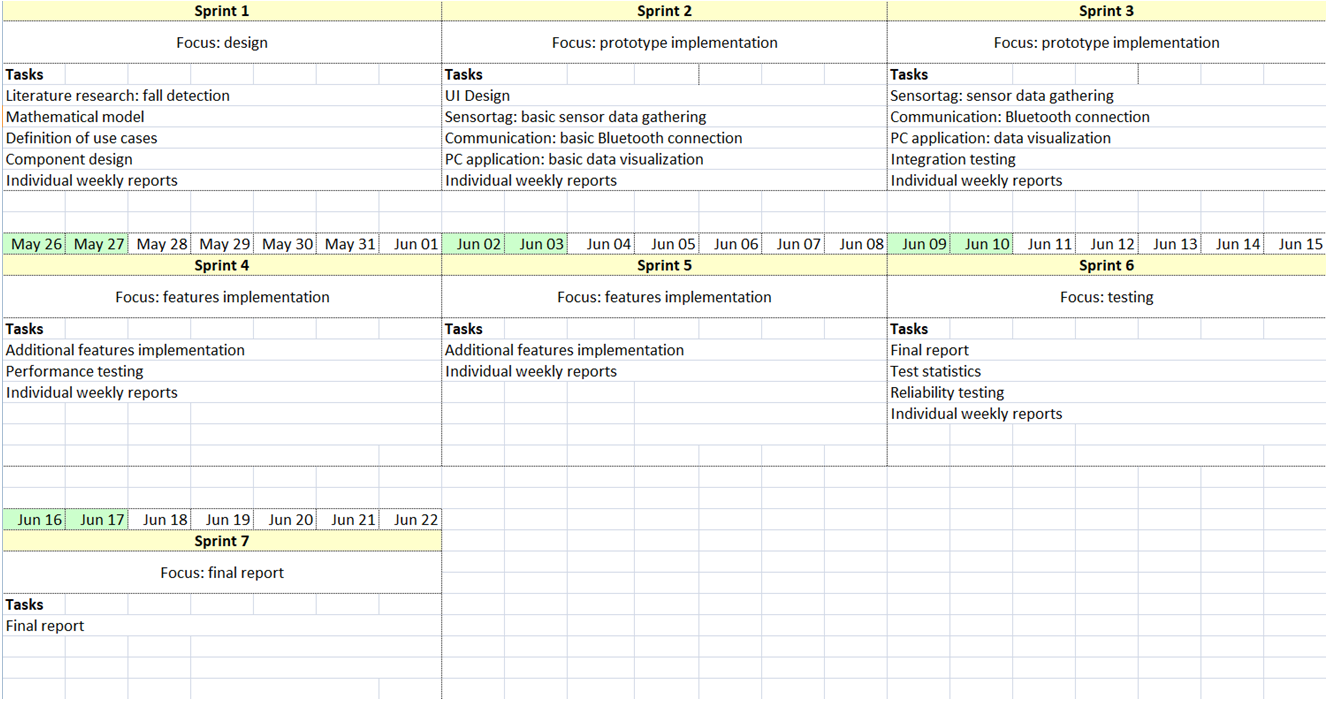
\includegraphics[scale=0.50]{images/Proj_Sched.png}
	\caption{Project Schedule}
	\label{img:Proj_Sched}
\end{figure}
\FloatBarrier

\subsection{Responsibilities of the Team Members}

All team members will assume several roles during the project. However, each person has been assigned a main role, making him or her the coordinator of all the individual efforts for a specific subject. 
\FloatBarrier
\begin{table}[h]
	\centering
	\caption{\textbf{Roles of the Team Members}}
	{\renewcommand{\arraystretch}{2}%
		\begin{tabular}{ | l | l | }
			\hline
			\textbf{Name} & \textbf{Main Role} \\ \hline
			Raul Bertone & Project Manager, Scrum Master \\ \hline
			Elis Harruni & Lead Java Developer \\ \hline
			Muyassar Kokhkharova & Statistics, UI Designer \\ \hline
			Saidar Ramazanov & Mathematical Model \\ \hline
			Xhoni Robo & Lead C Developer \\ \hline
	\end{tabular}}
\end{table} 

\clearpage
\FloatBarrier
\subsection{Project Risk Analysis}
\FloatBarrier
\begin{figure}[!h]
	\centering
	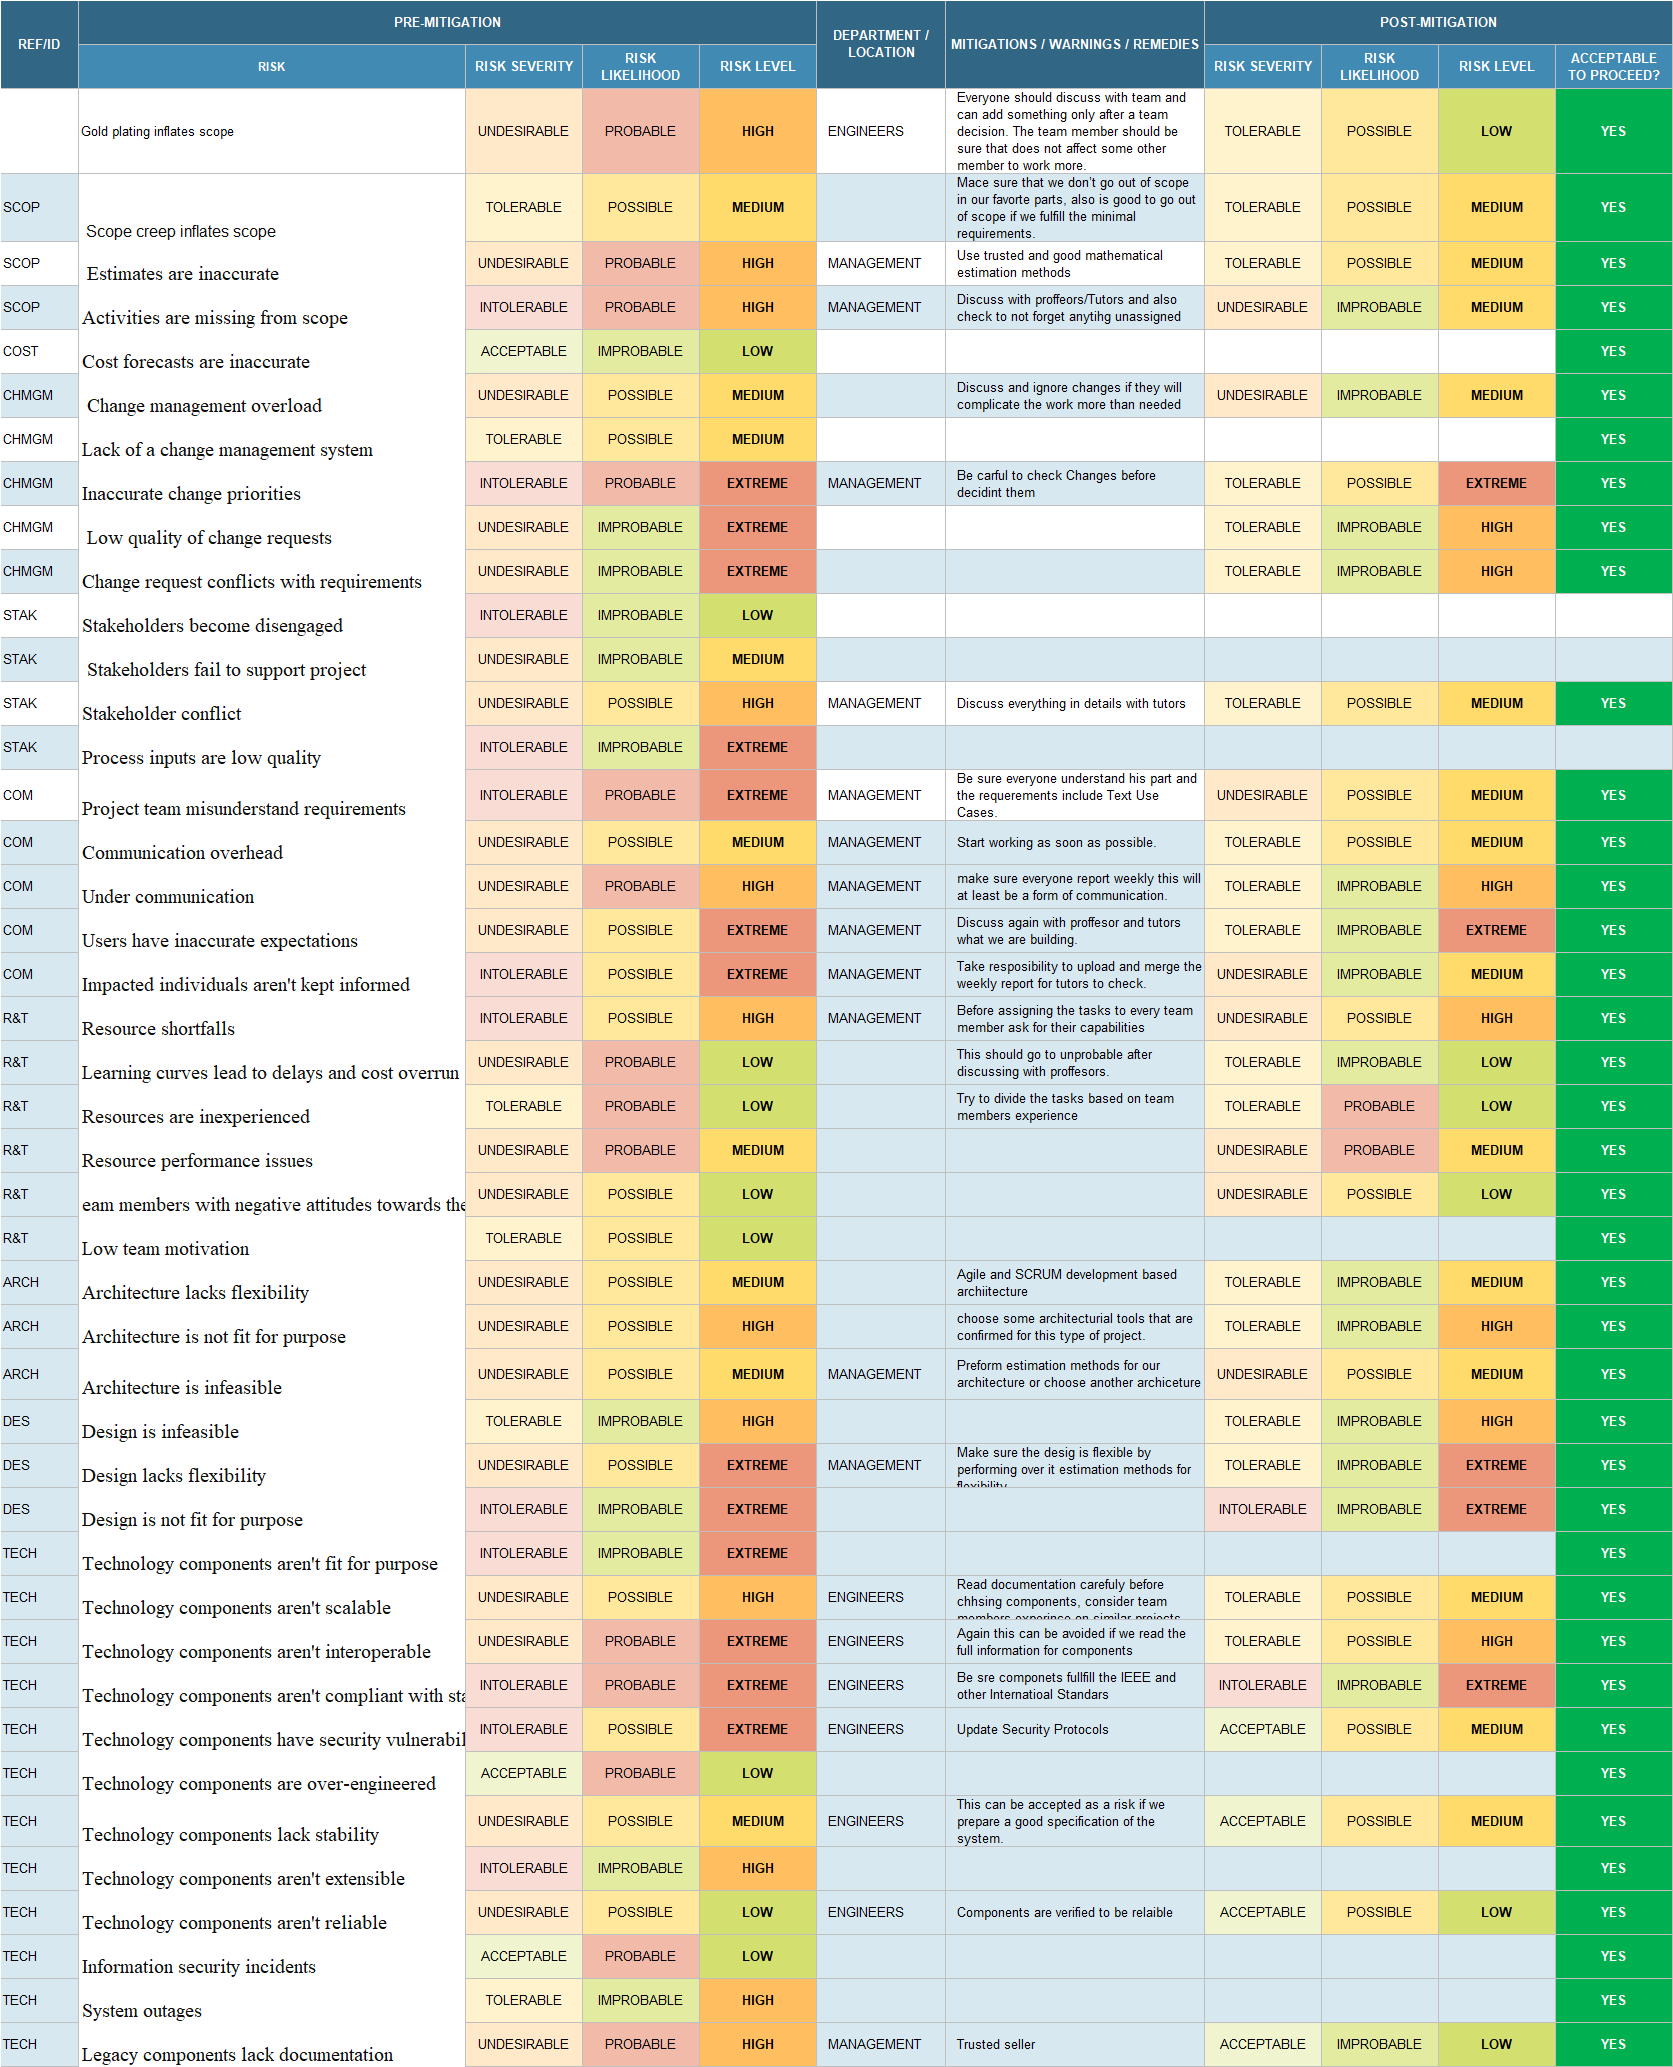
\includegraphics[scale=0.38]{images/Risk_Man_Matrix.png}
	\caption{Risk Management Matrix}
	\label{img:Risk_Man_Matrix}
\end{figure}
\FloatBarrier
\clearpage

\FloatBarrier
\begin{figure}[!h]
	\centering
	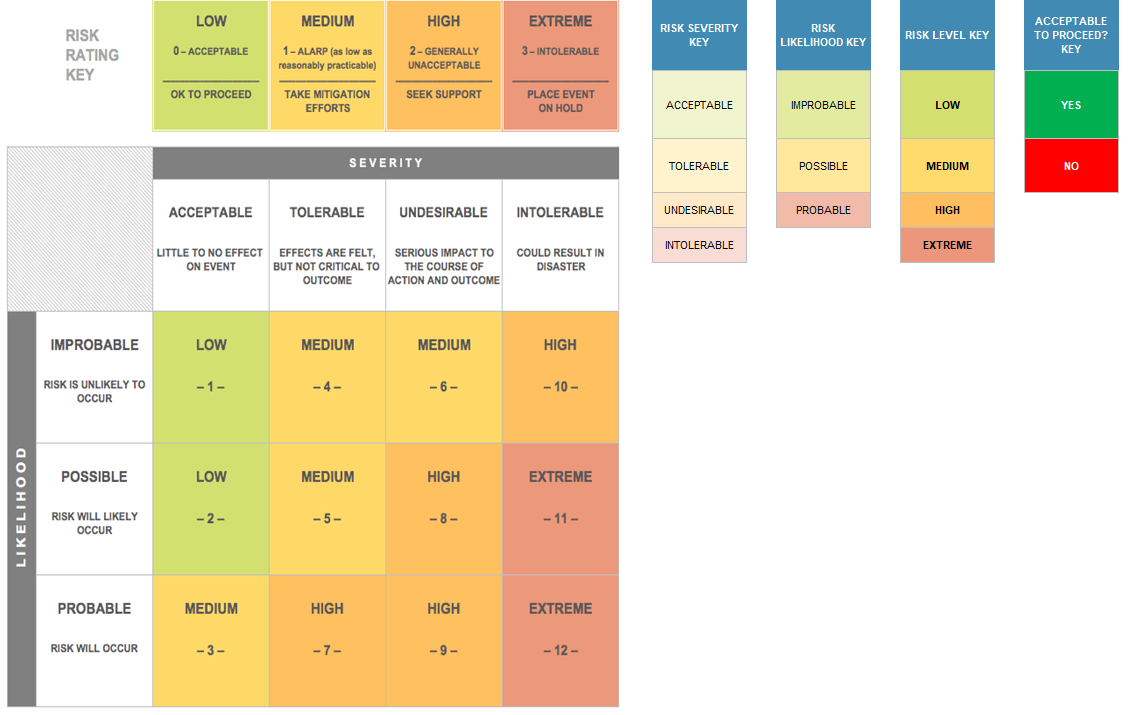
\includegraphics[scale=0.5]{images/Risk_Man_Key.png}
	\caption{Risk Management Matrix Key}
	\label{img:Risk_Man_Key}
\end{figure}
\FloatBarrier

\subsection{Setup and Description of Development Environments}
\textit{SensorTags}
\\The development for the SensorTags (and if necessary for the Launchpad) will be in C. For it we will use Texas Instrument’s own Code Composer Studio as well as the toolchain provided by Texas Instruments.\\
\\\textit{PC Application}
\\The PC application will be implemented in Java. For its development we will use Eclipse as an IDE, Junit for unit testing.
All mentioned software are available for both Linux and Windows, so we will leave the choice of an OS open for each team member (none makes use of MacOS). Additionally, the choice of Java as the implementation language allows the deployment and testing of the PC application on all OSs.\\
As a version control system software we selected git, and, based on this, GitHub as an online shared repository. All common artifacts (source code, documentation, etc.) will be uploaded there. In the root folder a readme file will describe the intended\\\\

\vskip 3cm 

use of the different folders. The master branch is protected from accidental modifications by requiring the use of pull-requests for its update.\\
The repository can be found at the following address:\\ \url{https://github.com/raulbertone/SSNS}
\\We integrated GitHub into our Slack group to be timely informed about commits performed by other team members.

\section{Functional and Non-Functional Requirements}
\subsection{Functional Requirements}
\begin{enumerate}
		\item Two CC2650 SensorTags are acting as peripherals and sending periodically acceleration and gyroscope data to the PC.
		\item A PC application should be able to connect simultaneously to multiple peripherals via BLE.
		\item A PC application should be able to receive sensor data (accelerometer and gyroscope) in real time.
		\item Data visualization. Line graphs with accelerometer and gyroscope data received from SensorTag.
		\item The graph should depict the average value of received sensor data within the offset time.
		\item Possibility to enter User‘s general information.
		\item Possibility to calibrate system thus differentiate between sudden movements like walking the steps and free fall.
		\item Main UI with basic control functions for operator working with a PC application.		
	\end{enumerate}


\subsection{Non-Functional Requirements}
\begin{enumerate}
	\item User general Information is a pop up window and it should contain:
	\begin{itemize}
		\item First Name
		\item Last Name
		\item Date of Birth
		\item Gender
		\item Address
		\item Mobile phone number of the User
		\item Blood Type
		\item Contact Person1 (In case of fall this Person will be contacted.)
		\item Contact Number1 (Phone number of a Contact Person1.)
		\item Contact Person2 (In case of fall and if Contact Person1 is not replying this Person will be contacted.)
		\item Contact Number2 (Phone number of Contact Person2.)
		\item Contact Person3\* (In case of fall and if Contact Person1 and Contact Person2 are not replying this Person will be contacted.)
		\item  Contact Number 3\* (Phone number of Contact Person3.)
		\item Save button to save changes
	\end{itemize}
	\item Application Settings is a pop up window containing the following information:
	\begin{enumerate}
		\item Offset with default value of 0.25 seconds.
		\\(Graphs of gyroscope and accelerometer will be updated every offset time with average values of gyroscope and accelerometer received during offset time.)
		\item Delta for fall detection
		\\(While falling values of accelerometer will gain acceleration and then will be equal to null. If delta of accelerometer received from sensor is bigger than configured delta in settings it will mean that the person has probably fallen. The duration of free fall is also important because we have to differentiate between	sudden movements like walking the steps and free fall, the duration will be different although delta values might be the same. While falling values of gyroscope will change and after reaching the 			ground values will be in horizontal position.)
		\item Set Default button\\
		 (After clicking on it, all the default values will be set and Settings pop up window will remain open.)
		 \item Save button\\
		 (After clicking on save button, all the changes will be saved and Settings pop up window will remain open.)
		 \item Cancel Button\\
		 (Cancel changes)
		 \item Close button
		 (Clicking on close button will close Application Settings pop up window) 
	\end{enumerate}
	\item In Main UI:
	\begin{enumerate}
		\item Graphs with Accelerometer and Gyroscope data.
		\item Accelerometer and Gyroscope data in the graphs will be updated at the same offset time.
		\item Buttons connect/disconnect(to establish the bluetooth connection).
		\item Buttons start/stop receiving gyroscope and accelerometer data.
		\item Button Clear graph.
		\item Label for Sensor Status (Connected to the sensor or No connection).
		\item Label for Fall Detection.\\
		(If fall is detected inscription about falling will be displayed.
		If not  inscription "Fall was not detected" will be displayed.)
		\item Label for "help requested"\\
		(If fall was detected and user did not pressed the button on SensorTag to report about False alarm inscription on requesting help will be displayed.)
		\item When the Sensor is not connected to the PC Application(e.g. when Data is not being received), than Buttons Start, Stop and Clear should be deactivated*
		\item Stop button is Activated when Start is pressed.
		\item "False Alarm" \\
		(When device senses a fall it beeps first and if button on 	SensorTag is not pressed quickly it calls for help)
	\end{enumerate}
\end{enumerate}

\section{Safety, Security and Reliability Requirements}
	For an application whose sole purpose is the detection of a person falling, it is important to ensure that it, at the very least, does what is required of it. However, it becomes of critical importance when paired with the fact that the user may be in danger following this fall. If this were a project made to be used for actual cases by hospitals for example, failure to correctly assess when a person is in danger may even be fatal. 
	\\Safety in this project translates to the protection of the hardware as well as software mechanisms that allow the fall to be detected. Preventing physical damage of the sensors is pretty self explanatory, and can be done by simply changing the design so that the fall itself would not be enough to break the sensors. As far as software is concerned, we need to ensure that the final application not only receives the data and correctly uses it, but also ensure that there are no interferences by other devices. In the case of low connectivity, the application should immediately notify the user. Lastly, the application should also ensure that it picks only the data received from the sensor tags. That way, there will be no issues with interference. Should anything not work as intended, the user should be notified immediately.\\
	Once safety and security is ensured, the final application needs to also be reliable. The most basic reliability requirement is to prevent the application of notifying us of events that are similar to a fall, but that provide no danger to the user. This includes physical activities such as walking, running and even jumping. Below is the full list of safety, security and reliability requirements:

\subsection{Safety Requirements}

	\begin{enumerate}
		\item Software correctly notifies when a person has fallen
		\item Software correctly notifies user when one or both sensor tags do not work
		\item Software or SensorTags correctly notify user when connectivity is low
		\item If transmission stops abruptly during an activity similar to a fall, count that as a fall
	\end{enumerate}


\subsection{Security Requirements}

	\begin{enumerate}
		\item Data is collected from the associated SensorTags
		\item Other devices cannot send data to the application
		\item If any interferences are detected, notify the user
	\end{enumerate}


\subsection{Reliability Requirements}

	\begin{enumerate}
		\item Software differentiates between falls and other similar activities
		\item Software does not crash during long sessions where a lot of data is streamed
		\item Software notifies user when the SensorTags are low on battery
		\item SensorTags only send the necessary data. Other sensors should be disabled
	\end{enumerate}

	
\section{Component Diagram}
\subsection{Introduction}

The diagram shows the main modules that make up our system: the Java application running onto the PC and the C application running on the two Sensortags.\\
The communication between the PC and the Sensortag happens over Bluetooth, with the former acting as central device and the latter as peripherals. The Sensortags don’t communicate directly with each other.

\FloatBarrier
\begin{figure}[!h]
	\centering
	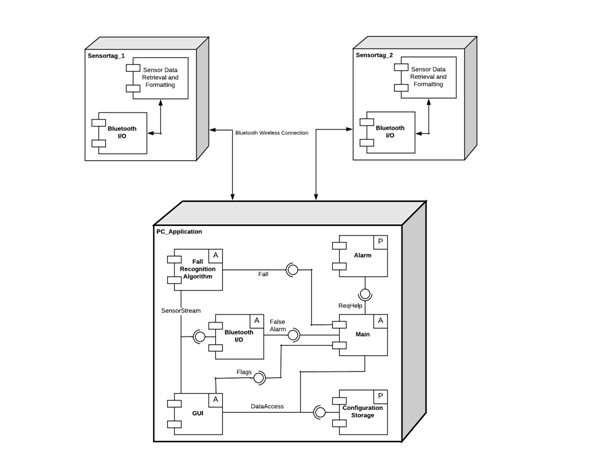
\includegraphics[scale=0.65]{images/Comp_Diag.png}
	\caption{Component Diagram}
	\label{img:Comp_Diag}
\end{figure}
\FloatBarrier

\subsection{Sensortags}
There are two logical modules in this application:

\begin{itemize}
	\item \textit{Sensor Data Retrieval and Formatting}. It activates and configures the necessary sensors and actuators, receives the measured values from the sensors and formats them appropriately before passing in to the second module;
	\item \textit{Bluetooth I/O}. Sets up the Bluetooth profile, services and characteristics; receives data from the previous module and forwards it to the PC\_Application.
\end{itemize}
It’s important to note that the modules described above don’t necessarily represent different files or libraries, but only different logical functions of the application, which might very well be implemented in the same file.

\subsection{PC\_Application}
The application is composed by six modules. The modules marked with an “A” are active modules, that is, they are executed within their own thread. “P” modules are instead passive, and their code is executed only when accessed by an active module.
\begin{itemize}
	\item \textit{Bluetooth I/O}. Manages the Bluetooth connection and receives the data from the Sensortags; sends an alarm when a Fall Event is detected;
	\item \textit{Fall Recognition Algorithm}. Fetches sensor data from the Bluetooth Input module and examines it to look for Fall Events. When one is detected, it informs the GUI module and sends an alarm to the Bluetooth I/O module; 
	\item \textit{GUI}. Displays the graphical user interface; fetches sensor data from the Bluetooth I/O module to produce the graphs; retrieves and saves configuration data in the Configuration Storage module;
	\item \textit{Main}. Contains the business logic of the application. When a Fall Event is detected by the Fall Recognition Algorithm module, raises the Fall Detected flag in the GUI and sends a false alarm request to the Sensortags; if the false alarm request is not answered, it reads the help data from the Configuration Storage, requests help through the Alarm module and raises the Help Requested flag in the GUI;
	\item \textit{Alarm}. Sends an “alarm”, simulated here by sending an email;
	\item \textit{File Access}. Reads and writes the configuration files.
\end{itemize}
On one hand, the separation into modules will allow the team to subdivide the development tasks and work in parallel, while on the other, the definition of formal interfaces will simplify coordination between this development efforts.
Like noted for the Sensortag application, the modules represent only a logical subdivision of the features, and don’t necessarily correspond to specific packages. However, is reasonable to expect that several of them will be implemented as independent packages. 

\subsection{Interfaces}
\textit{False Alarm}
\\Module:Bluetooth I/O
\\Input: control over the buzzer in the Sensortags
\\Output: events (presses) of button\_2 on the Sensortags
\\\\\textit{DataAccess}
\\Module: Configuration Storage
\\Input: write access to the configuration file(s)
\\Output: read access to the configuration file(s)
\\\\\textit{SensorStream}
\\Module: Bluetooth I/O
\\Input: none
\\Output: one data stream for each sensor
\\\\\textit{Fall}
\\Module: Main
\\Input: none
\\Output: fall event detected
\\\\\textit{ReqHelp}
\\Module: Alarm
\\Input: help message (email body); message address (email address)
\\Output: none
\\\\\textit{Flags}
\\Module: GUI
\\Input: “fall detected” status (Boolean); “help requested” status (Boolean)
\\Output: none

\section{Use Case Diagram}
\textit{Activate}: User presses button on SensorTag to turn it on. PC app connects to SensorTag and starts receiving data\\
\textit{Deactivate}: PC stops receiving data from SensorTag, disconnects from SensorTag and User presses button on SensorTag to turn it off\\
\textit{Out of Range}: PC app stops receiving data, loses connection and sends help request to Helper\\
\textit{Fall}: User falls, system recognizes fall and requests help\\
\textit{False Alarm}: User “falls”, system recognizes fall and receives False Alarm signal\\
\textit{Modify personal data}: User modifies his personal data and system saves changes\\
\textit{Modify calibration}:  User modifies calibration and system saves changes\\
\FloatBarrier
\begin{figure}[!h]
	\centering
	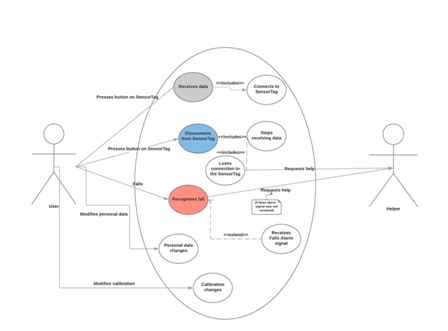
\includegraphics[scale=0.8]{images/Use_Case_Diag.png}
	\caption{Use Case Diagram}
	\label{img:Use_Diag}
\end{figure}
\FloatBarrier

\subsection{Sequence Diagrams}

\FloatBarrier
\begin{figure}[!h]
	\centering
	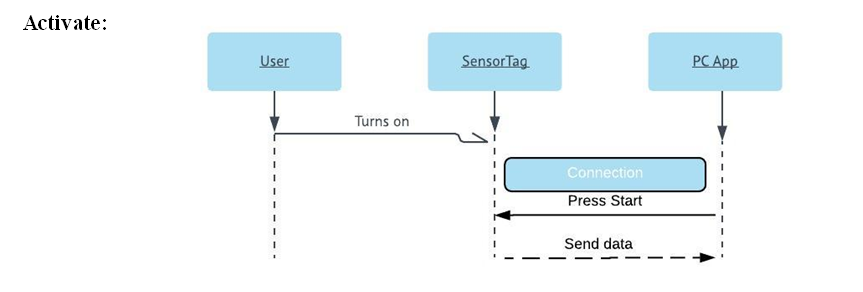
\includegraphics[scale=0.4]{images/Seq_Activate.png}
	\label{img:activate}
\end{figure}
\FloatBarrier

\FloatBarrier
\begin{figure}[!h]
	\centering
	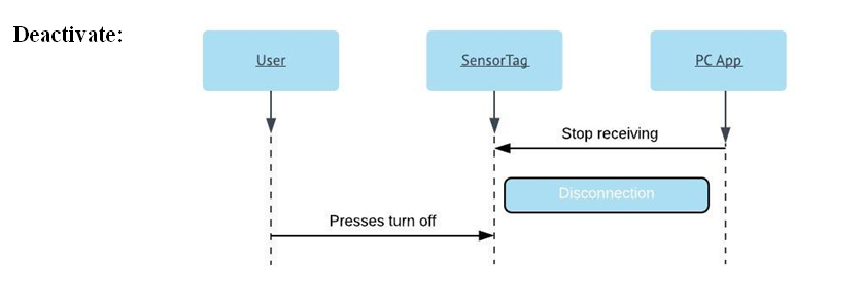
\includegraphics[scale=0.4]{images/Seq_Deactivate.png}
	\label{img:deactiv}
\end{figure}
\FloatBarrier

\FloatBarrier
\begin{figure}[!h]
	\centering
	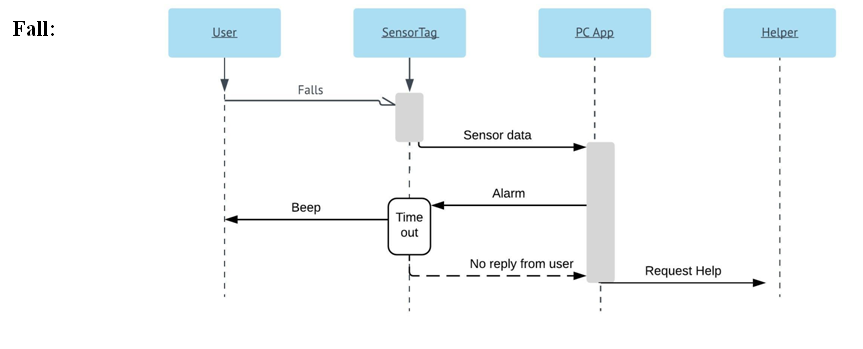
\includegraphics[scale=0.4]{images/Seq_Fall.png}
	\label{img:fall}
\end{figure}
\FloatBarrier

\FloatBarrier
\begin{figure}[!h]
	\centering
	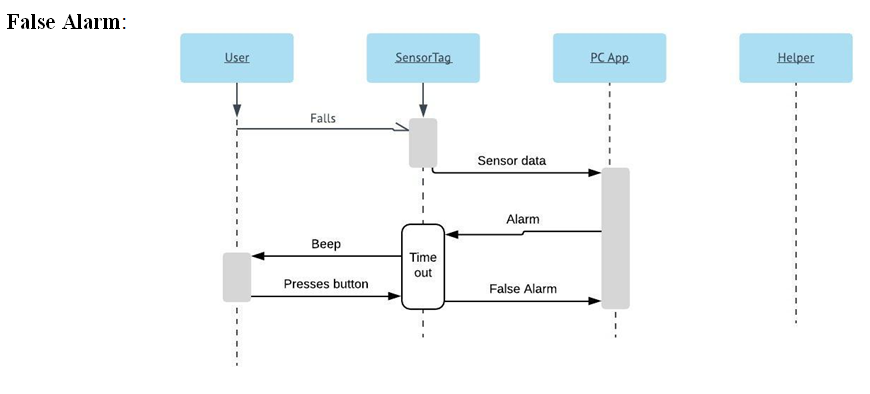
\includegraphics[scale=0.4]{images/Seq_FalseAl.png}
	\label{img:falseal}
\end{figure}
\FloatBarrier

\FloatBarrier
\begin{figure}[!h]
	\centering
	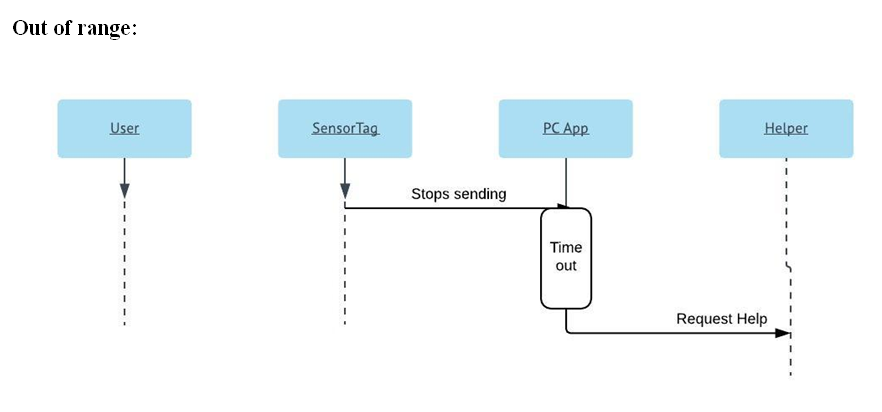
\includegraphics[scale=0.4]{images/Seq_OOR.png}
	\label{img:OOR}
\end{figure}
\FloatBarrier

\FloatBarrier
\begin{figure}[!h]
	\centering
	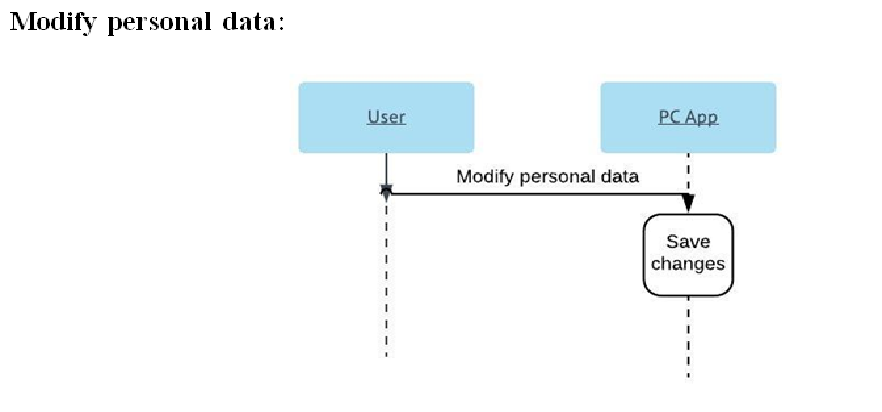
\includegraphics[scale=0.4]{images/Seq_Modify.png}
	\label{img:modpersdata}
\end{figure}
\FloatBarrier

\FloatBarrier
\begin{figure}[!h]
	\centering
	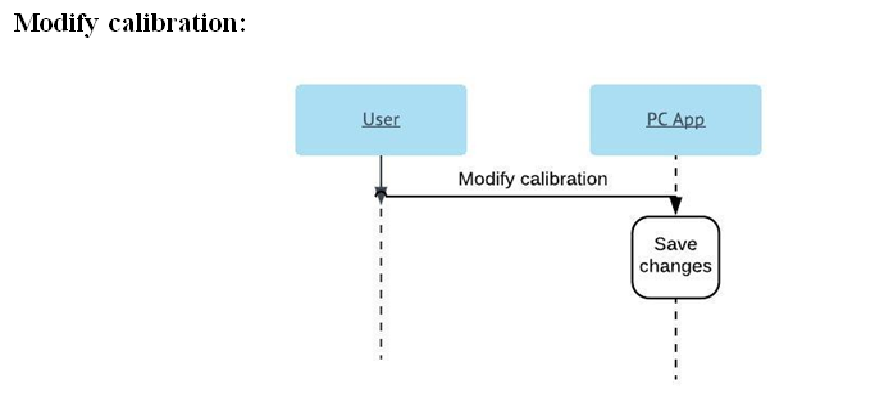
\includegraphics[scale=0.4]{images/Seq_Modify_Cal.png}
	\label{img:modcal}
\end{figure}
\FloatBarrier

\section{SensorTag Development}
\textbf{Function activation and deactivation:} we were able to deactivate the unused functions in the “proper” way, by adding the relevant pre-processor options: EXCLUDE\_OAD, EXCLUDE\_REG, EXCLUDE\_OPT, EXCLUDE\_BAR, EXCLUDE\_HUM, EXCLUDE\_TMP. In the same way we also activated the buzzer, with the option  Board\_BUZZER.\\\\
\textbf{Movement sensor configuration:} first, using the appropriate bitmask in the \textit{mpuconfig} variable, we were able to configure the movement sensor. In particular we set the sensitivity of the accelerometer to +/- 4G and we turned off the magnetometer.\\\\
\textit{mpuconfig = 0x1BF}\\\\
Additionally, we increased the update rate of the whole sensor to 20Hz (instead of the standard 1Hz).\\\\
\textbf{I/O service:} to be able to control the buzzer (and LEDs) remotely via Bluetooth, we modified the I/O service configuration.\\\\
\textit{ioMode = 1}\\\\
At the moment, this concludes the development on the SensorTags.

\subsection{Dead SensorTags}
We did some investigation on why the SensorTags often stopped working after flashing. We found out that, on some computers, flashing by connecting the Debugger module via USB 3.0 would “kill” the Sensortag (it would then only work while powered through the Debugger itself, but not on battery alone). To avoid this, it was enough to flash via a USB 2.0 port instead of 3.0. However, to bring back a “killed” Sensortag it is first necessary to flash the hex file using the Flash Programmer 2 (again, only via USB 2.0).

\subsection{Desktop Application Development}
During the past two weeks since the last report, the team has completed a primary version of the \textit{Alarm Module} and of the \textit{Configuration Module}. The first is able to send an email to one or more contacts to request assistance. The second stores all the information needed by the application. This information is of two kinds:  
\begin{enumerate}
	\item user data and contact information for the helpers
	\item calibration and settings information for the sensors
\end{enumerate}

\section{Implementation of Math Model}
On the previous week, the Mathematical logic of the accelerometer fall detection was implemented. The architecture of the implementation was easy and reliable for the first look. Program starts a thread when the function of the maths model is triggered by main package and it gets new measurements from sensors. However, it was found that the amount of measurements per second is too high. It means that there will be 25 threads each moment. Also, the minimum fall time is 450 ms, consequently the program can skip calculations for 10 measurements. Finally, the mathematical model will not care about calculations for 500 ms, during that time the Mathematical class will only add new measurements into the array of data. It is obvious that there will be only two threads of calculations in one moment. This brings less memory usage and increases of speed of the application.\\\\
Another point was made, that the thread should be started inside Mathematical class, instead of starting it outside. It brings more flexibility for the program, because the application will just trigger functions of this class, and is not worried with what happens inside this class.

\section{Gyroscope}
To use only the accelerometer is not enough to detect the fall. The application should include protection from making wrong decisions. That is why it was important to figure out the logic of additional part in Mathematical package.\\\\
First, the application should store data from sensors for the Gyroscope the same way as for the Accelerometer part in parallel. Secondly, the main mathematical part (accelerometer) should detect a fall. If it happens, the main part should trigger the method of the Gyroscope class and gives time stamps of the start and end of the fall. Then, the Gyroscope part is going to the previous measurements, when falling begins and the accelerometer has approximately -1 g on OZ axis. Between these two timestamps, the application started to measure the angle of the fall on two axis. If the composition angle of the two axis is equal to: $$90 \pm 35 \pm 180 * n, where\ n \in Z,$$
then it means that the patient is laying and the Gyroscope class proofs the fall.\\\\
The main problem of it is to understand from what point of time the application should start calculations of the patient tilt.

\section{Machine Learning}
On one of the previous team meetings, it was stated that our team would implement Machine Learning only if we will have enough time at the end of the project. On the previous week, it was decided that the application should be more reliable for decisions. That is why it was figured out that the application should also calculate angle of the patient during the fall.\\\\
To minimize risks, a decision was made to check how Machine Learning can be implemented in our app. If ML is faster to implement it makes more sense to change the whole strategy of the Mathematical part. However, after research, it revealed that in order to implement ML, the team faces with several problems:
\begin{itemize}
	\item State a model for ML;(It is easy to do)
	\item Convert the data from sensors to data, which can be understandable by ML (it will be the biggest problem, because data should be pre-processed. It means that all data that the application has should be converted to boolean data. Consequently, ML cannot decide if it's a fall or not depending on exact data from sensors)
	\item •	Implement learning techniques for ML.
\end{itemize}
Model for ML can contain the following boolean fields: 
\begin{itemize}
	\item isImpact – absolute value of acceleration more than \textbf{2g}
	\item isLayng – absolute value of acceleration after 400 ms on OX and OY axis is equal to \textbf{1g}
	\item isMoving – absolute value of acceleration still more than \textbf{1,5 g}
	\item isRotating – angular speed is more than normal
\end{itemize}

\begin{table}[!h]	
	\begin{center}
		{\renewcommand{\arraystretch}{2}%
		\begin{tabular}{|c|c|c|c|c|} 
			\hline
			\textbf{isImpact} & \textbf{isLayng} & \textbf{isMoving} &\textbf{isRotating} & \textbf{Fall} \\ [0.5ex] 
			\hline
			1 & 1 & 0 & 0 & 1 \\ 
			\hline
			1 & 1 & 0 & 1 & 1 \\
			\hline
			0 & 0 & 1 & 1 & 0 \\
			\hline
			0 & 1 & 0 & 1 & 0 \\  [1ex]
			\hline  
		\end{tabular}
	}
	\end{center}
\end{table}
As the result, ML in fall detection can do only a small part of the work that is why it is not effective to implement it at the field of study. 

\section{Graphical User Interface} 
To implement GUI based on the mock up made earlier, JavaFX Scene Builder\cite{JavaFX} was used. JavaFX Scene Builder is a tool that lets users design a JavaFX application's UI. UI components can be draged and dropped to a work area, modify their properties and at the end we will have FXML code for the created layout generated automatically. The result is a FXML file that can be combined with a Java project by binding the UI to the applications logic. \\\\
In the first version of GUI we have main window with area for Accelerometer and Gyroscope graphs and buttons: Connect, Disconnect, Start(receiving data), Stop(receiving data), Clean. In the menu bar we have User General Information, Settings and Close buttons. In User General Information the user should fill in the form with his data and the contact person`s data. We are planning to modify the Settings window and we will discuss it on our weekly group meeting.

\section{Research and analysis of the Multi\_Role Application}
Due to the constraint as a result of the short amount of time until the end of the project, choosing the best approach is the difference between a successful application and the failure of the project. That is why, while exploring the possibility of using a Java application to connect to the SensorTag, still through the use of the LaunchPad, it would be necessary to continue the research on the Multi\_Role application, as well as understanding how to change the code in order to be able to adapt it to our current needs. Since the documentation on the Multi Role application on the internet is lacking, the best approach would instead be to look at the code and try to understand how it works. To help, we are trying to compare the Multi\_Role application to the Host\_Test application.\\

\subsection{Multi\_Role issues that prevent implementation}
Firstly, the Multi\_Role application is, as mentioned previously, hardly documented. This made it a challenge at first to understand how the application works. After setting up the environment using PuTTY, we were able to use the application. After running the application, everything seemed to work except for the GATT Read/Write operation. In order to track the execution process, we used the debugger feature on Code Composer Studio to track the path of the code, with the hope that it would eventually lead to the function, or at least the file, that handled the Read/Write operation. However, because the application requires input from the LaunchPad buttons in order to execute its functions, the debugger would stop right after the BIOS was initialized, and even though the code would run, no input would be recognized. The alternative approach meant looking at the code itself, and tracking the definition of the methods to get to the right place. Doing so eventually led to the answer that contained the Read/Write function, which consisted of basically an IF statement, that counted the times the operation was successful. Therefore, the main problem became being able to implement a working Read/Write operation.\\

\subsection{Comparing Multi\_Role to Host\_Test}
Due to the constraint as a result of the short amount of time until the end of the project, choosing the best approach is the difference between a successful application and the failure of the project. That is why, while exploring the possibility of using a Java application to connect to the SensorTag, still through the use of the LaunchPad, it would be necessary to continue the research on the Multi\_Role application, as well as understanding how to change the code in order to be able to adapt it to our current needs. Since the documentation on the Multi Role application on the internet is lacking, the best approach would instead be to look at the code and try to understand how it works. To help, we are trying to compare the Multi\_Role application to the Host\_Test application.\\\\
Unlike the Multi\_Role, the Host\_Test application has a higher amount of documentation available. However, the amount is almost infinitely bigger, and finding the small piece of information required to make the implementation of the application is just as difficult as it was for the Multi\_Role. So far, a quick skim of the main documentation given by TI gave us a basic understanding of how the Host\_Test works. However, little of help was given regarding the Read/Write in particular, at least as far as the implementation of it is concerned. More progress will be done until we have a final solution.\\

\subsection{TinyB}
I found a promising project by Intel called TinyB. This project aims at providing a simple Blutooth API for IOT devices, and it also came with an example specifically using a Sensortag.\\\\
The host part of the Bluetooth stack is implemented in C++, while the API is available in C++ and Java. Since we wanted to use Java, the build and deployment process turned out to be less than straightforward in that it involved using make, a tool tailored for use with C/C++, for an hybrid C++-Java project.\\
Moreover, I had no experience interfacing Java code with other languages, a process that requires the use of the Java Native Interface (JNI).\\
After overcoming all these hurdles, I was presented with a very simple and API and, within minutes, I was able to connect and operate a single Sensortag. Unfortunately there was no build-in way to connect at the same time to more than one Bluetooth server device. From the experience of other users online, I gathered that it is indeed possible, although complex, unreliable and undocumented. In particular everybody seemed to experience constant disconnections when more than one device was connected.\\
At this point I decided to resume my search, in the hope of finding a simpler solution.


\subsection{Kura}
The Eclipse project called “Kura”, a framework for the server side of IOT applications, seemed a good candidate. It contains a Bluetooth LE API which is actually internally based on TinyB. The advantage here is twofold: all the development happens in Java, with the JNI well hidden under several abstraction layers; a Sensortag example is available with a comprehensive API, much more powerful than TinyB on its own. Also there is the hope that multi-device connection would be handled automatically by the framework.\\\\
In general, if we were not so low on time, I wouldn’t have considered Kura as a solution because, while specifically dedicated to IOT development, it is extremely heavyweight. Kura is an OSGI application and requires therefore an OSGI container to be run (for example Eclipse Equinox). This implies the use of pure Linux has the OS (Android in not compatible). This does not fit our scenario as it would require a powerful, and probably non-battery powered device as a Bluetooth base station (at best a Raspberry Pi or similar).\\\\
The next step would be to start working on the available Sensortag example and, again, see if it is possible and easy to connect more than one device.\\

\section{Desktop Application Development}\cite{vendor}\cite{devguide}\cite{userguide}
\textit{This is the report for 4 week since Elis could not report the previous time.}
First a recap of what I was doing I am working all the time with establishing BLE  connection and creating a network to read the required data from the sensors.\\
I started directly with multi\_role project that was suggested to me I could connect tow Slaves to the lunchpad (Master) but to discover Characteristics and read/write I could not do. That happened because the Write/read function of multi role project was not implemented. Considering to implement that function and solve the problem I decided not to do it because of my restricted knowledge on C and C++ from this decision starts the work of this 4 weeks.\\\\
First 2 weeks using host\_test application with lunchpad again as a master I created a network for 1 sensor as a slave reading data and saving them in queue to print on console after that just to see the messages.\\
The implementation was done by the help of Java library to read and write to a serial COM port called jssc.jar.\\
\begin{figure}[!h]
	\centering
	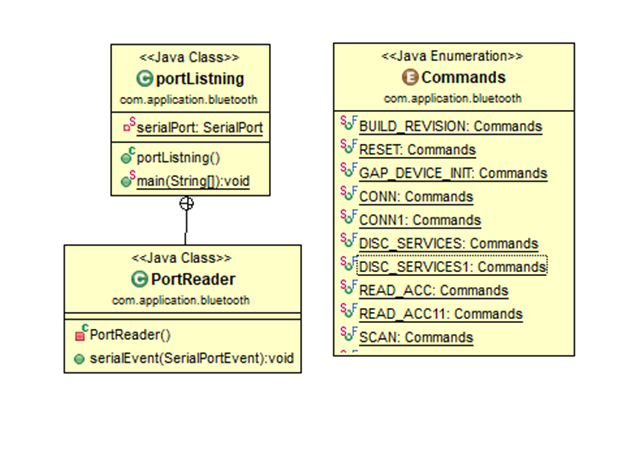
\includegraphics[scale=0.50]{images/UML1.png}
	\caption{UML diagram for the first prototype of Network system in JAVA}
	\label{img:UML1}
\end{figure}
\\First I needed only this three classes portListning PortReader that is a private inner class of port listning and an Enumeration for some commands that I need to send to lunchpad.\\
In the port listning Class the main method search for available COM ports and print them after that it ask you what port want to connect and open. After that activating a SerialPortEvent to the opened port will notify this thread every time that an event is happening to the port write/read.
On the PortReader Class that implements SerialPortEvent Interface implementing the required method serialEvent I only catch read events so when the lunchpad is sendig me data and I just print the hexadecimal Sring in console to check the data.\\
The time consuming part was Creating the so called Commands I started to build commands using TI BLE Vendor Specific HCI Reference Guide BLE5 Version 1.0.0.\\
Creating commands like that was taking a lot of time and I figured out another method sniffing the port with a port sniffer application while I used BLE device monitor for getting data.
Then o got all the writing commands with the help HCI Reference Guide I could translate all messages so I Go only the commands that I need to read from Accelerator. Here I was trying to get data only from Accelerator then later will think for Gyroscope.\\
A the end I could get data for my Application but I need to translate those data and to parse in the way I get a use of them.\\\\
This 2 week I continue on building the NS (Network System) part of SSNS.\\
\begin{figure}[!h]
	\centering
	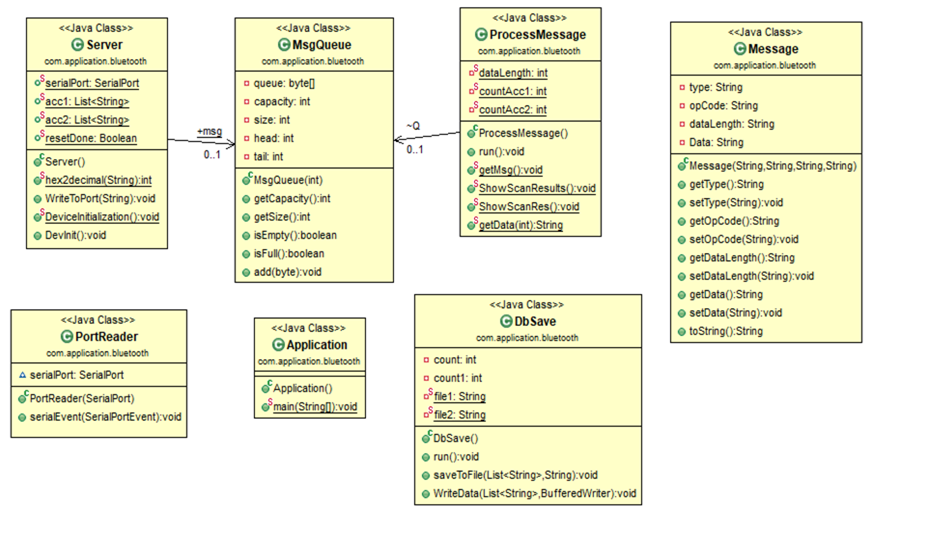
\includegraphics[scale=0.40]{images/UML2.png}
	\caption{New current Application UML diagram.}
	\label{img:UML2}
\end{figure}
\\This is the auto generated UML diagram from an Eclipse plugin that's why there are some relations missing without a detailed explanation this UML is not understandable because of missing elements.
Also here the Commands Enumeration is missing because is very big for the figure.\\
Here we have now 7 classes this is developed from the first Application in previous weeks with 3 classes PortReader is the same but instead of a private inner class now I use Aggregation and Inheritance to implement the same thing. “portListning” was not named good for Java convention by mistake and with the new ideas I got a new name for it that is Server and the main() method now is in a new class Called Application that is somehow the user interface for now(Consloe view).
Now I don’t print the message on the Console when I get an event but insert the byte array to a Byte Queue I implemented and to process the Messages and to parse and translate the messages I use a new thread that gets the data from Queue so I get lower chances to interrupt or to put the main Thread  in a lot of work and risk losing data.\\
I have defined a structure of the every message with the help of TI BLE Vendor Specific HCI Reference Guide BLE5 Version 1.0.0.\\
DbSave class is just a class to save Accelerator data in 2 different files for different sensors.
So with this Structure I can connect 2 sensortags and get data from them in the same time.
Apart for the successful work I was working on developing a python script to read the data from sensor and also with android code from TI but I then gave another try to this before finding a solution on one of those 2.\\


\section{Implementation of Math Model}
On previous weeks was implemented additional functional of Gyroscope method of Fall Detection. As it was mentioned on the last report, the logic of work is:\\\\
First, application should store data from sensors for Gyroscope like for the accelerometer part in parallel mode. Secondly, main mathematical part (accelerometer) should detect a fall. If it happens, the main part should trigger method of Gyroscope class and gives time stamps of the beginning and ending of the fall. Then, Gyroscope part is going to the previous measurements, when falling is started and accelerometer has approximately -1 g on OZ axis. Between these two timestamps, application started to measure angle of the fall on two axis. If composition angle of two axis is equal to:
$$90 \pm 35 \pm 180*n, where n \in Z,$$
then it is mean that patient is laying and Gyroscope class proofs the fall.\\
First problem was to state the timeframe when the fall was. In that point, algorithm looking for the last measurements of \textbf{-1 g} on OZ axis and states it as beginning of fall. Then the end of fall is stated by time when the impact was proceed. By this, we can state the timeframe of the fall for the Gyroscope algorithm.  However, if the measurement of OZ axis is 0 g it means that the user was laying before the fall.\\\\
One of the main problem during the implementation was that the program could not change array of measurements during the computations. That is why there was implemented footprint of the measurements. It brings some disadvantages, as the program should store a lot of information for computations. Nevertheless, it is one solution, which can be done in case to do not lose important measurements from SensorTag.\\\\
Finally, the architecture of the Maths logic now contains three classes:\\
\begin{itemize}
	\item Mathematics – contains main thread of computations, creating stamp of Gyro and Accelerometer objects inside the thread, and contains main static variables like impact power, laying acceleration;
	\item Gyro – contains measurements from sensor, functions off adding new measurements, thread of Gyro computations;
	\item Accelerometer - contains measurements from sensor, functions off adding new measurements, can trigger Gyro method to start its thread.
\end{itemize}

%----------------------------------------------------------------------------
% Bibliography
%----------------------------------------------------------------------------	
\printbibliography
\end{document}
%----------------------------------------------------------------------------
